\begin{figure}[htb]
	\centering
	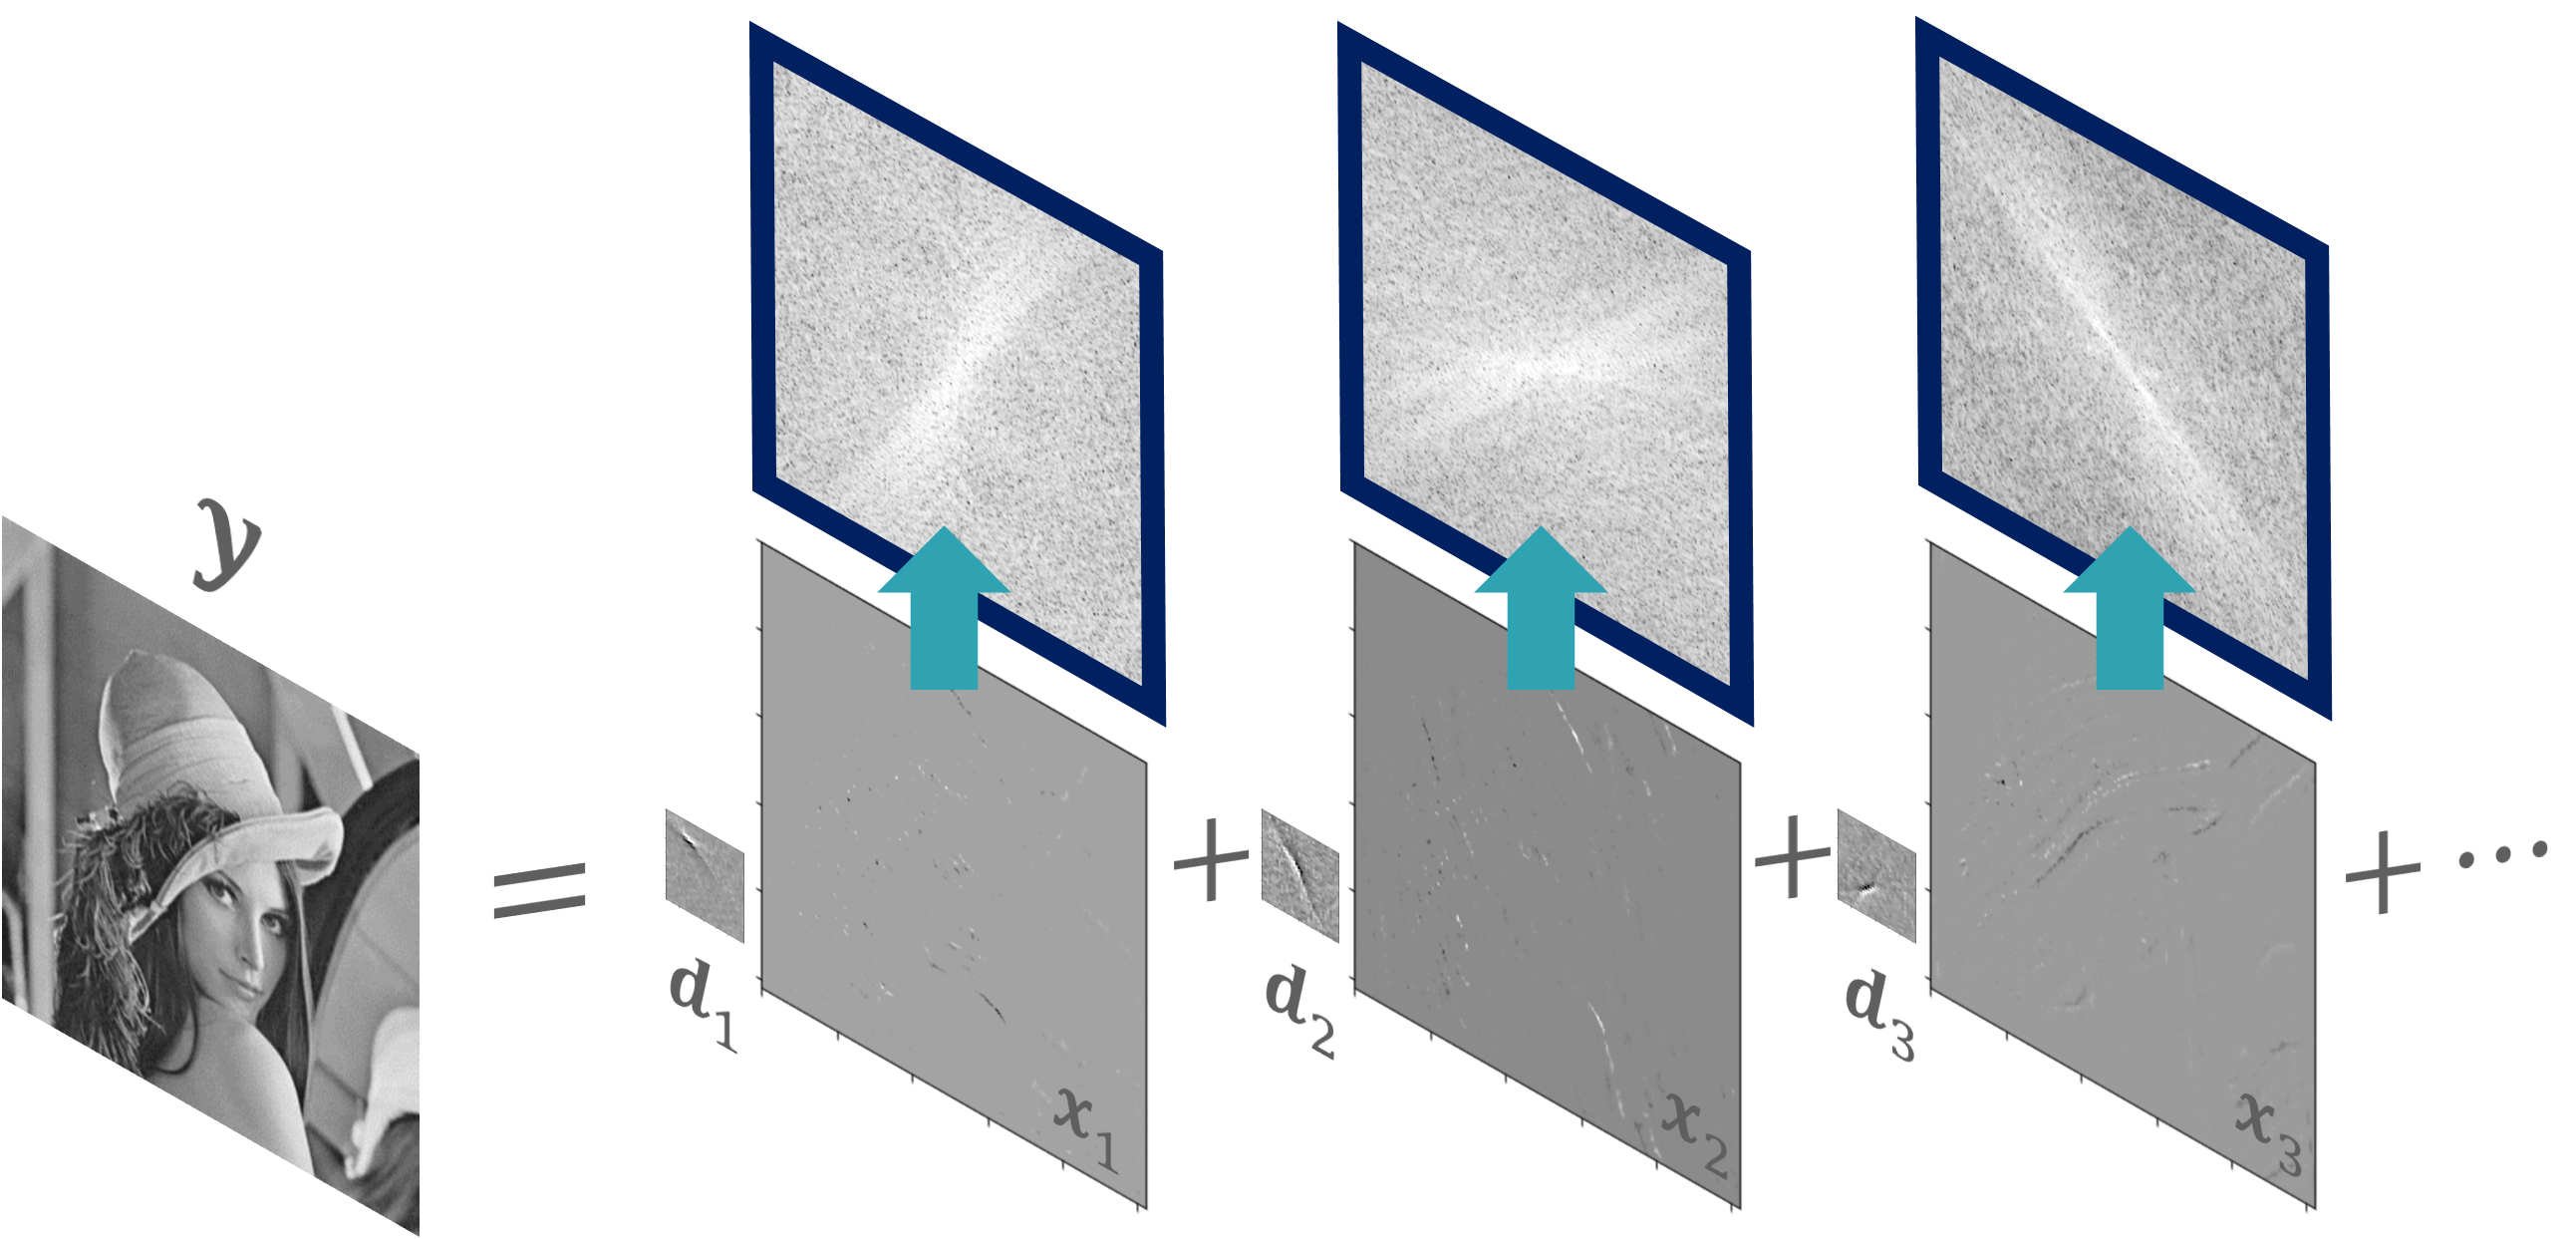
\includegraphics[width=0.7\linewidth]{image/power-spectrum}
	\caption{提案法で使用する特徴(図中の太枠部分)}
	\label{fig:power-spectrum}
\end{figure}

畳み込み辞書学習におけるフィルタは,エッジやテクスチャなどの局所的な特徴をとらえるのに対し,係数マップはフィルタの示す特徴が入力信号のどの部分に顕在しているのかを示す.
したがって,入力信号がシフト変動を受けるとき,係数マップも近しい変動を受けると考えられる.
そこで本研究では,疎な係数マップのパワースペクトル(図\ref{fig:shift})を特徴として用いることで,シフト変動に頑健な特徴を設計する.
パワースペクトルはその信号に含まれる各周波数成分の振幅を示すものである.
これにより,データセット内の各データ間の位置ずれに対して頑健な特徴抽出が可能となる.

\begin{figure}[htb]
	\centering
	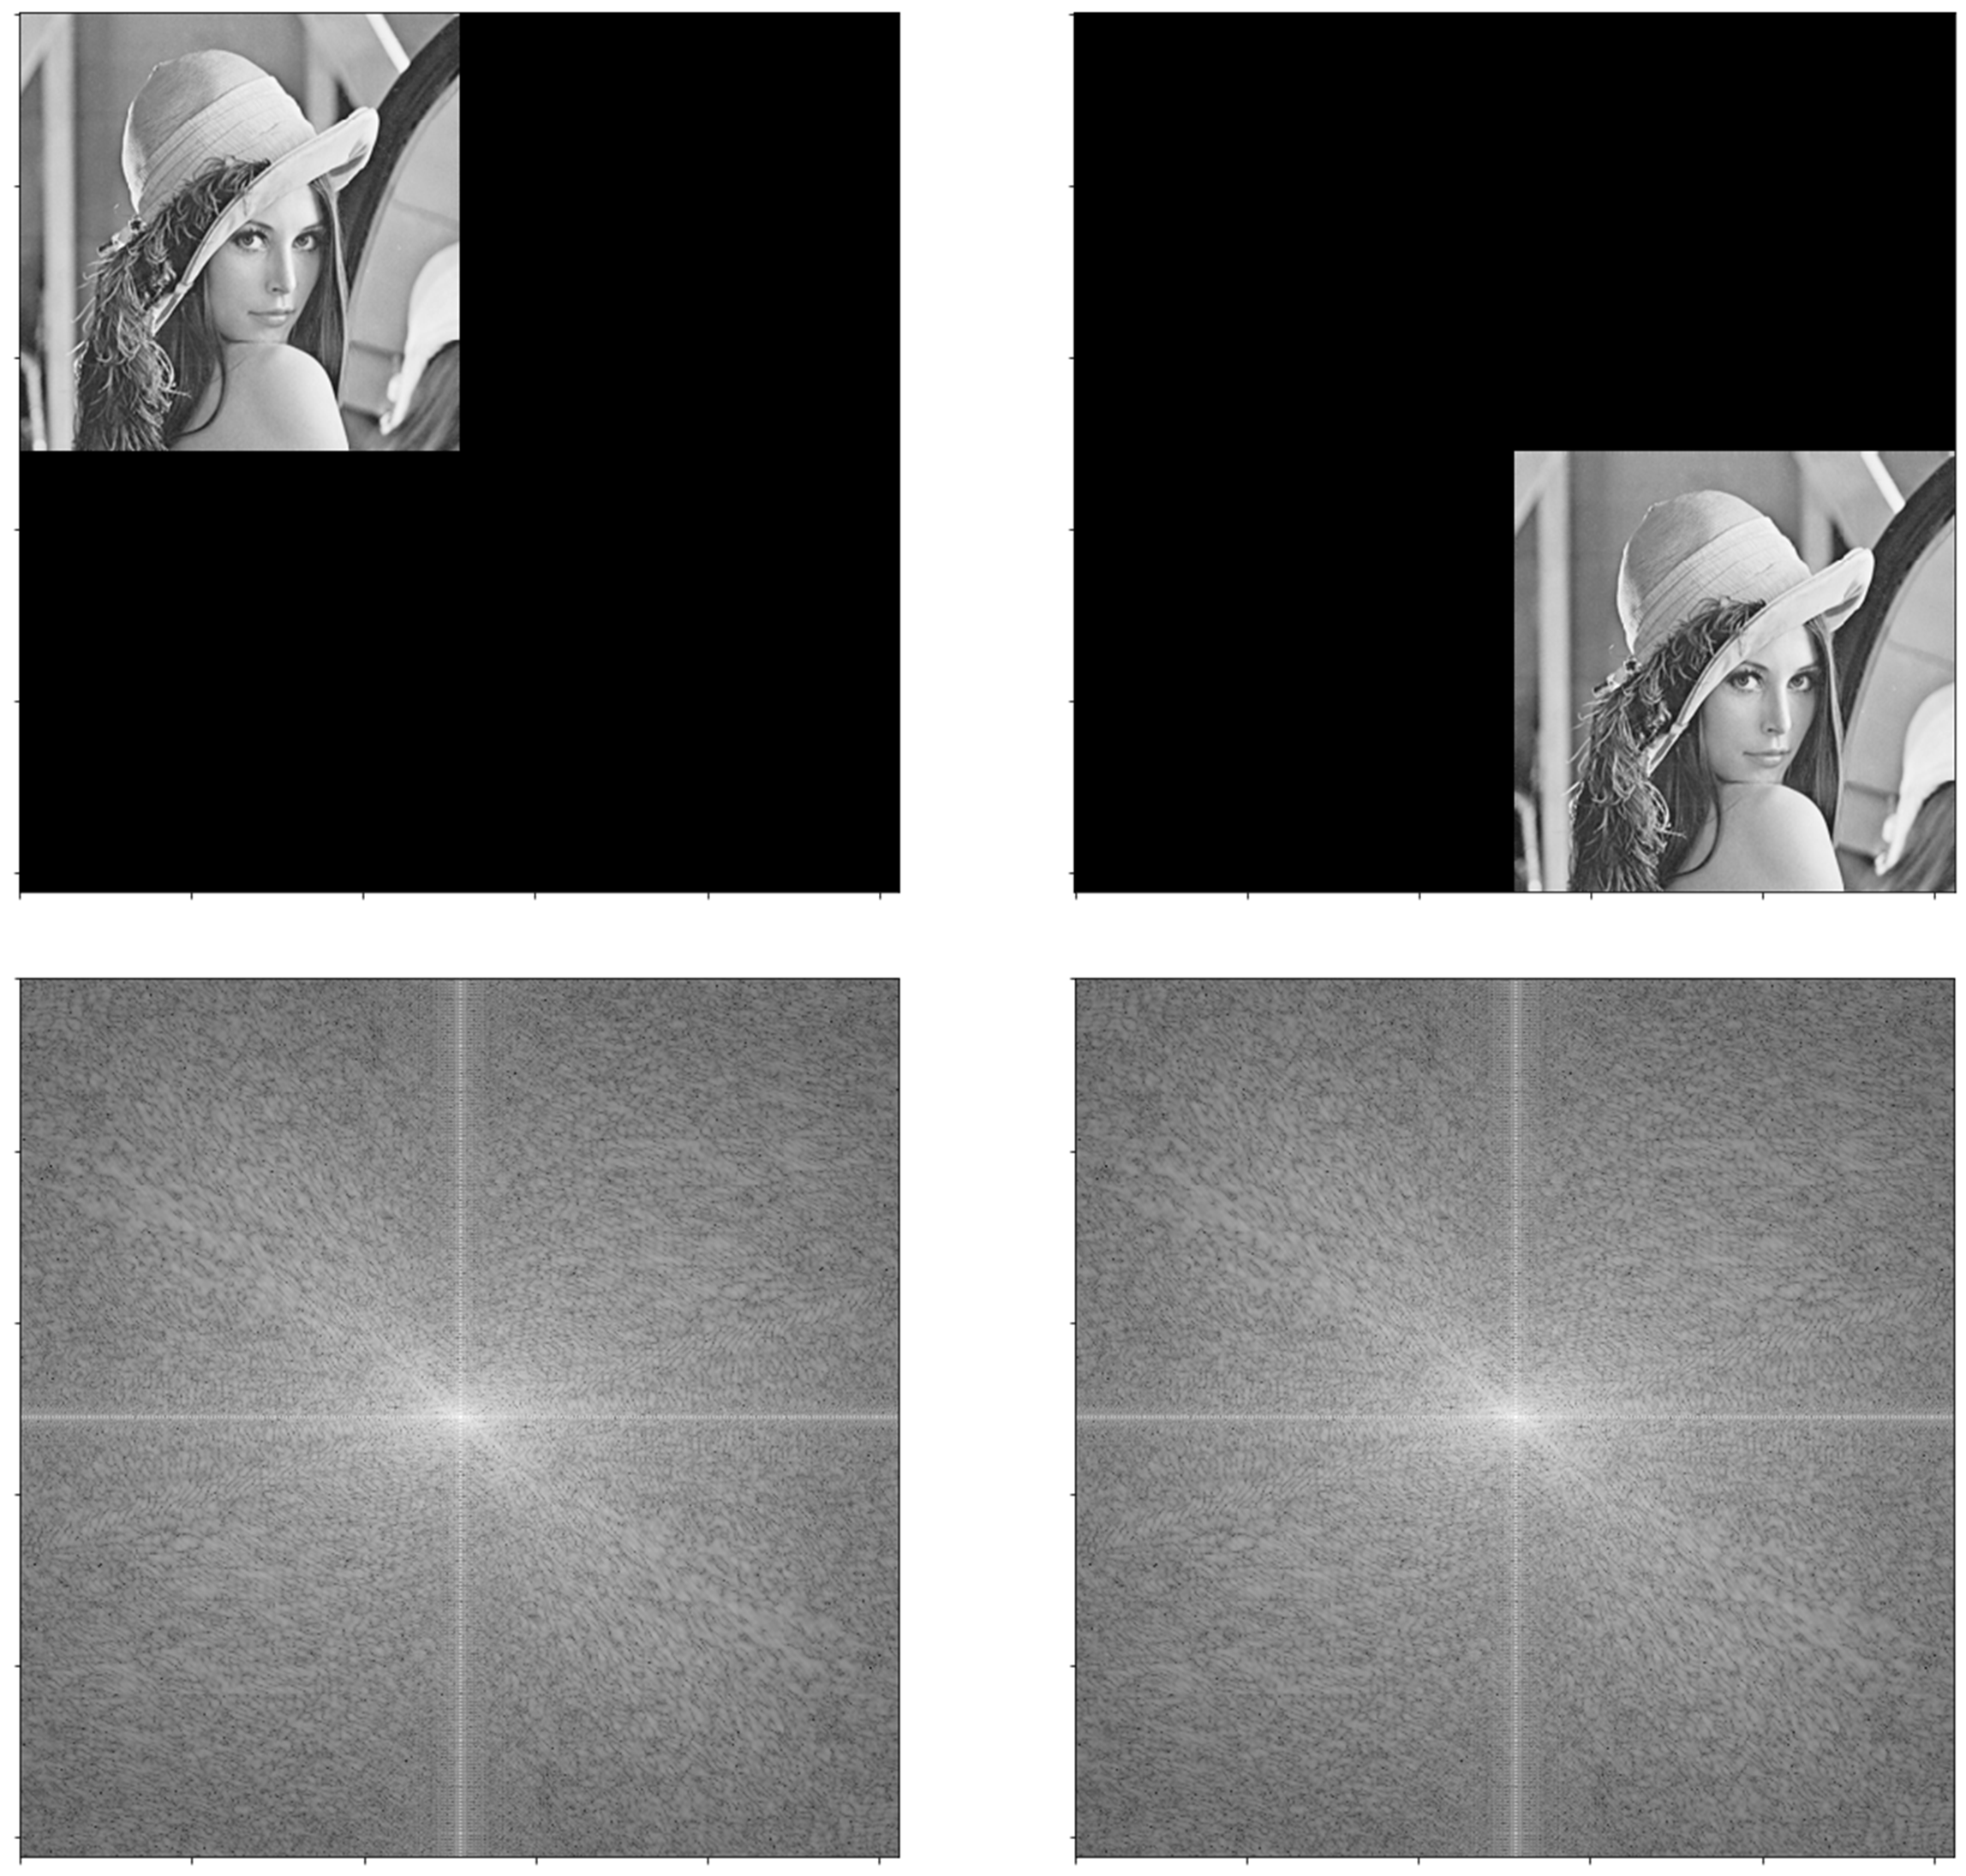
\includegraphics[width=0.7\linewidth]{image/shift}
	\caption{シフト変動させた信号に対するパワースペクトル}
	\label{fig:shift}
\end{figure}

また,本研究ではパワースペクトルの非負値性を利用し,部分空間法ではなく,錐制約を課した部分空間法を分類問題に適用する.